\documentclass[11pt]{article}

\usepackage[margin=1in]{geometry}
\usepackage[T1]{fontenc}
\usepackage[utf8]{inputenc}
\usepackage{lmodern}
\usepackage{graphicx}
\usepackage{amsmath,amssymb,amsfonts}
\usepackage{algorithmic}
\usepackage{textcomp}
\usepackage{xcolor}
\usepackage[hidelinks]{hyperref}
\usepackage{booktabs}
\usepackage{multirow}
\usepackage[numbers]{natbib}
\usepackage{tikz}
\usetikzlibrary{positioning, arrows.meta}

\hyphenation{poly-chron-isa-tion}

\begin{document}

\title{\Large\textbf{Permutations Are All You Need:\\Lookup-Table Transformers with Ranking Embeddings}}

\author{Eugene Izhikevich \and Vyacheslav Kluchnikov \and Anatoly Starostin}
\date{}

\maketitle

% ======================================================================
\begin{abstract}
Modern transformers represent tokens as real-valued vectors and manipulate them through matrix multiplications.
In this work we explore an alternative representation grounded in the \emph{Spiking Manifesto}~\cite{ref:manifesto}: we encode information in the \emph{relative ordering} (permutation) of embedding dimensions rather than in their magnitudes, and replace matrix multiplications with differentiable lookup tables (LUTs) indexed by pairwise comparisons.
We keep the high-level transformer architecture intact --- attention, residual connections, softmax --- and change only the underlying embedding language and the projection mechanism.

We evaluate several LUT-based transformer variants on a byte-level language modelling benchmark (FineWeb, context 32, vocab 257) against a 4.87M-parameter vanilla baseline achieving cross-entropy 1.356.
Our best \emph{Ranking Attention} model reaches 1.381 (gap 0.025), albeit at substantially higher parameter count.
A more parameter-efficient variant reaches 1.408 with 17.7M parameters.
We further introduce \emph{HyperLUT}, a differentiable module that maps binary comparison features through a two-layer MLP, combining permutation semantics with efficient GPU execution.

Our results demonstrate that permutation-based embeddings can approach the quality of magnitude-based representations for sequence modelling, while opening a path toward hardware implementations that require only comparators and table reads instead of multiply-accumulate units.
\end{abstract}

\medskip
\noindent\textbf{Keywords:} lookup tables, permutation embeddings, ranking attention, spiking neural networks, transformers, polychronisation


% ======================================================================
\section{Introduction}
\label{sec:intro}

The standard transformer architecture~\cite{ref:vaswani} represents each token as a real-valued vector in $\mathbb{R}^d$ and transforms sequences through linear projections and dot-product attention.
The information carried by each embedding is encoded in the \emph{magnitudes} of its components: two embeddings are similar when their dot product is large.
This paradigm has proven extraordinarily successful, but it is tightly coupled to matrix multiplication as the fundamental computational primitive.

The \emph{Spiking Manifesto}~\cite{ref:manifesto} proposes a radically different view.
In biological spiking neural networks, information is encoded in the \emph{relative timing} of spikes --- which neuron fires before which --- rather than in firing rates or voltage magnitudes.
This \emph{permutation-based} encoding offers factorial capacity ($n!$ distinguishable patterns for $n$ neurons) compared to the exponential-in-precision capacity of real-valued vectors, and the underlying computation can be realised through \emph{lookup tables} (LUTs) indexed by pairwise timing comparisons~\cite{ref:manifesto}.

In this work we take these ideas from the biological domain and apply them to practical sequence modelling.
We ask: \emph{can we build a transformer that operates on permutation embeddings and uses lookup tables instead of matrix multiplications, while achieving competitive language modelling performance?}

Our approach preserves the high-level transformer structure --- layers, attention, residual connections, softmax --- and replaces only two things:
\begin{itemize}
    \item \textbf{The embedding language:} low-dimensional vectors ($d=32$) where information resides in the relative ordering of dimensions, not their magnitudes.
    \item \textbf{The projection mechanism:} differentiable lookup tables indexed by pairwise comparisons, replacing dense linear projections.
\end{itemize}

We present three families of LUT-based transformers of increasing sophistication:
(1)~\emph{Simple LUT transformers} that replace all projections with LUTs;
(2)~\emph{Ranking Attention transformers} that project queries and keys into a pairwise-comparison feature space where Kendall-$\tau$ correlation reduces to cosine similarity, enabling standard scaled dot-product attention on permutation features;
and (3)~\emph{HyperLUT transformers} that replace discrete table lookup with a two-layer MLP operating on binary comparison features, combining permutation semantics with efficient GPU execution.

All experiments are conducted on a byte-level language modelling benchmark using a subset of the FineWeb dataset, allowing direct comparison with a standard transformer baseline.\footnote{All code and experiments are available at \url{https://github.com/anatoli-starostin/spiky}.}


% ======================================================================
\section{Background}
\label{sec:background}

\subsection{Permutation Embeddings vs.\ Magnitude Embeddings}

In a standard transformer, an embedding $\mathbf{x} \in \mathbb{R}^d$ carries information in the values of its components.
Two embeddings interact through their dot product $\mathbf{x}^\top \mathbf{y} = \sum_i x_i y_i$, which depends on the magnitudes $x_i, y_i$.

A \emph{permutation embedding} carries information in the \emph{relative ordering} of its components.
Given $\mathbf{x} \in \mathbb{R}^d$, the ordering $\sigma_\mathbf{x}$ is the permutation that sorts $x_{\sigma(1)} \leq x_{\sigma(2)} \leq \cdots \leq x_{\sigma(d)}$.
Two permutation embeddings are similar when many pairs agree on which component is larger.
This is precisely the Kendall-$\tau$ rank correlation:
\begin{equation}
    \tau(\mathbf{x}, \mathbf{y}) = \frac{1}{\binom{d}{2}} \sum_{i < j} \mathrm{sgn}(x_i - x_j) \cdot \mathrm{sgn}(y_i - y_j).
    \label{eq:kendall}
\end{equation}

The encoding capacity of permutation embeddings is $d!$ (the number of distinct orderings), which grows factorially.
For $d = 16$, this gives $16! \approx 2 \times 10^{13}$ distinguishable patterns encoded in roughly $\log_2(16!) \approx 44$ bits.
A magnitude-based vector in $\mathbb{R}^{16}$ with float32 precision can represent $2^{512}$ distinct states --- vastly more --- but this capacity depends entirely on the ability to distinguish fine numerical differences.
In practice, operations like normalisation, quantisation, and additive noise destroy magnitude information, collapsing many of those $2^{512}$ states into equivalence classes.
The permutation capacity, by contrast, is robust: it depends only on the relative ordering, which is invariant to scaling, shifting, and any monotonic transformation of individual dimensions.

As shown in~\cite{ref:manifesto}, the number of $\varepsilon$-distinguishable vectors in $\mathbb{R}^n$ (the ANN capacity) scales as $e^{c(\varepsilon) \cdot n}$ where $c(\varepsilon) \sim \varepsilon^2$, while the combinatorial capacity of ordering-based representations scales as $m^n$ where $m \sim 1/\varepsilon$.
Since $1/\varepsilon \gg e^{\varepsilon^2}$ for any practical precision, the ordering-based capacity dominates.


\subsection{Lookup Tables as Computational Primitive}

Following~\cite{ref:manifesto}, we replace matrix multiplications with lookup tables indexed by pairwise comparisons.
A single lookup table $S$ with $n_c$ \emph{anchor pairs} operates as follows:

\begin{enumerate}
    \item \textbf{Compare:} For each anchor pair $(a_k, b_k)$, $k = 1, \ldots, n_c$, compute the binary comparison $c_k = \mathbf{1}[x_{a_k} > x_{b_k}]$.
    \item \textbf{Index:} Form the integer index $j = \sum_{k=1}^{n_c} c_k \cdot 2^{k-1} \in \{0, \ldots, 2^{n_c} - 1\}$.
    \item \textbf{Lookup:} Retrieve the weight vector $S_j \in \mathbb{R}^{n_\mathrm{out}}$ from the table.
\end{enumerate}

The output of a multi-table module with $T$ tables is the sum:
\begin{equation}
    \mathbf{y} = \sum_{t=1}^{T} S_{t, H_t(\mathbf{x})}
    \label{eq:lut}
\end{equation}
where $H_t(\mathbf{x})$ is the hash function (comparison + indexing) for table $t$.

This operation requires only \emph{comparators} and \emph{table reads} --- no multiply-accumulate units.
Each table stores $2^{n_c} \times n_\mathrm{out}$ parameters but accesses only \emph{one row} per input, giving low inference-time memory bandwidth.

We refer to $n_c$ as \textbf{nap} (number of anchor pairs) and $T$ as \textbf{tph} (tables per head) throughout this paper.
These are the two fundamental parameters controlling the expressiveness and capacity of LUT-based layers.


\subsection{Differentiable Training of Lookup Tables}
\label{sec:surrogate}

The lookup function~\eqref{eq:lut} is piecewise constant with zero gradients almost everywhere.
To enable gradient-based training, we use \emph{surrogate gradients} via an uncertainty function.

For each comparison $\delta_k = x_{a_k} - x_{b_k}$, we define an uncertainty:
\begin{equation}
    U(\delta) = \frac{1}{2(1 + |\delta|)}
    \label{eq:uncertainty}
\end{equation}
which is large near the decision boundary ($|\delta| \approx 0$) and vanishes for confident comparisons.
During the backward pass, the gradient through each anchor pair involves two quantities computed by the downstream projection layer: a \emph{gradient carrier} for the main table entry, $g = \sum_o \frac{\partial L}{\partial y_o} \cdot S_{j,o}$, and for the closest alternative entry, $g' = \sum_o \frac{\partial L}{\partial y_o} \cdot S_{j',o}$, where $j'$ is the index obtained by flipping the least-confident bit.
The gradient with respect to input $x_{a_k}$ is then proportional to $(g - g') \cdot U'(\delta_k)$, where $U'$ is the derivative of the uncertainty function.
The paired anchor $x_{b_k}$ receives an equal and opposite contribution~\cite{ref:manifesto}.


% ======================================================================
\section{Experimental Setup}
\label{sec:setup}

All experiments share the same data, tokenisation, and evaluation protocol to ensure fair comparison.

\subsection{Dataset and Tokenisation}

We use a 234\,MB subset of the FineWeb dataset~\cite{ref:fineweb}, a curated collection of English web text.
Tokenisation is byte-level: each input byte maps to one of 256 token IDs, plus a special beginning-of-sequence token (BOS), giving a vocabulary of $V = 257$.
The context length is $T = 32$ tokens.

\subsection{Evaluation Metric}

We report \emph{validation loss}: mean per-token cross-entropy on 10,000 held-out test regions, computed after each 1,000 training steps.

\subsection{Training Protocol}

Unless otherwise noted, all models are trained with Adam~\cite{ref:adam} using learning rate $10^{-3}$, cosine annealing with 10\% linear warmup (decaying to 10\% of peak), and batch size 128 for 100K steps.
Training is performed on a single NVIDIA H100 80GB GPU.

\subsection{Vanilla Transformer Baseline}

Our reference model is a standard causal transformer with embedding dimension $d = 256$, 4 attention heads, 6 layers, and feed-forward expansion factor 4, totalling 4.87M parameters.
After 100K training steps it achieves validation loss \textbf{1.356}.
This serves as the target for all LUT-based models.


% ======================================================================
\section{LUT Transformer Design Principles}
\label{sec:design}

Before presenting specific architectures, we describe the design principles common to all LUT-based transformers in this study.

\subsection{Data Flow Similarity}

We are not attempting to reinvent sequence modelling.
The transformer is a proven, universal architecture for this task, and we preserve its structure entirely.
The \emph{only} things we change are:
\begin{itemize}
    \item The \textbf{embedding language}: low-dimensional vectors ($d = 32$) where information resides in the relative ordering of dimensions, not their magnitudes.
    \item The \textbf{projection mechanism}: lookup tables indexed by pairwise comparisons, replacing dense linear layers.
\end{itemize}

All structural blocks remain the same.
In every LUT transformer variant, we work with sequences of token embeddings, organise computation into layers with residual connections, compute attention scores followed by softmax, and apply an unembedder that returns logits over the vocabulary.
This deliberate isomorphism ensures that any performance difference is attributable to the change in representation and projection mechanism, not to architectural novelty.

\subsection{Positional Encoding}
\label{sec:positional}

Positional encoding in low-dimensional permutation embeddings requires special care.
In standard transformers with $d = 256$ or higher, adding a positional vector ($\mathbf{x} + \mathbf{p}$) is a small perturbation that preserves most of the information in $\mathbf{x}$.
At $d = 32$, however, additive positional encoding can significantly alter the relative ordering of dimensions, destroying the permutation structure that carries the token's identity.

We explored several approaches:
\begin{itemize}
    \item \textbf{Additive PE:} $\mathbf{x} + \mathbf{p}$ --- standard approach; disrupts ordering at low $d$.
    \item \textbf{Concatenation:} $[\mathbf{x}, \mathbf{p}]$ --- dedicates separate dimensions to position; preserves content ordering.
    \item \textbf{Positional buckets:} Discrete bucket indices multiplying the effective LUT table size; used in early experiments.
    \item \textbf{Relative positional embeddings (RelPE):} Learned vectors indexed by distance $|i - j|$; concatenated with pair embeddings in score computation.
    \item \textbf{Per-layer positional summation:} Separate learned positional vector per layer, added to Q/K input before LUT projection; viable when the LUT itself is comparison-based and tolerant of additive shifts.
\end{itemize}

Empirically, concatenation and RelPE consistently outperform additive PE at $d = 32$: no PE gives val loss 1.929, additive PE gives 1.493, and concatenation gives 1.684 (on a simpler architecture where concatenation doubles input dimension).
The choice between these strategies depends on the specific architecture, as discussed in the following sections.

\subsection{The nap/tph Tradeoff}
\label{sec:nap_tph}

The two fundamental parameters of a LUT layer are:
\begin{itemize}
    \item \textbf{nap} (number of anchor pairs): the number of pairwise comparisons per table, determining the table size $2^{\mathrm{nap}}$ entries.
    \item \textbf{tph} (tables per head): the number of tables whose outputs are summed per head, determining the model's capacity.
\end{itemize}

At fixed parameter budget ($\sim$5M), we sweep this tradeoff (Table~\ref{tab:nap_tph}).

\begin{table}[!t]
\caption{nap vs.\ tph tradeoff at $\sim$5M parameters}
\label{tab:nap_tph}
\centering
\begin{tabular}{ccrr}
\toprule
nap & tph & Entries/table & Val loss \\
\midrule
7  & 32   & 128 & 1.827 \\
5  & 128  & 32  & 1.729 \\
\textbf{4}  & \textbf{256}  & \textbf{16}  & \textbf{1.706} \\
3  & 512  & 8   & 1.706 \\
2  & 1024 & 4   & 1.719 \\
1  & 2048 & 2   & 1.965 \\
\bottomrule
\end{tabular}
\end{table}

Many small tables consistently outperform few large tables in terms of validation loss, with $\mathrm{nap} = 3\text{--}4$ as the sweet spot.
However, this tradeoff has an important hardware dimension: large tables (high nap) access \emph{fewer rows} per forward pass, offering lower memory bandwidth.
A model with nap=10 and tph=128 reads 128 rows per head per input, while nap=3 with tph=512 reads 512 rows.
On specialised hardware where table reads dominate latency, fewer large tables may be preferable despite worse validation loss.

\subsection{Anchor Pair Sampling Policies}
\label{sec:sampling}

The choice of \emph{which} input dimensions each table compares affects performance (Table~\ref{tab:sampling}).
We evaluate several sampling policies:
\begin{itemize}
    \item \textbf{Balanced:} Random permutations ensuring each dimension appears equally often across tables.
    \item \textbf{Connected/Disconnected:} Pairs that share or avoid sharing indices within each table.
    \item \textbf{Full coverage:} All $\binom{d}{2}$ unique dimension pairs are tiled across tables, ensuring complete pairwise coverage.
\end{itemize}

\begin{table}[!t]
\caption{Anchor pair sampling policies (nap=4, tph=256)}
\label{tab:sampling}
\centering
\begin{tabular}{lr}
\toprule
Policy & Val loss \\
\midrule
Random (balanced) & 1.706 \\
Connected & 1.721 \\
Disconnected & 1.687 \\
\textbf{Full coverage} & \textbf{1.684} \\
\bottomrule
\end{tabular}
\end{table}

Full coverage gives consistent improvement, and we adopt it for all subsequent experiments.
For $d = 32$ with nap=4, full coverage requires $\mathrm{tph} \geq \lceil\binom{32}{2} / 4\rceil = 124$ tables per head to cover all 496 unique pairs.


% ======================================================================
\section{Simple LUT Transformers}
\label{sec:simple_lut}

Our first approach replaces all learned projections in the transformer with LUT modules while keeping the overall architecture intact.

\subsection{Architecture}

The \emph{LUT Transformer V3} uses the following per-block structure:
\begin{enumerate}
    \item \textbf{Score LUT:} For each causal pair $(i, j)$ with $j \leq i$, concatenate $[\mathbf{x}_i, \mathbf{x}_j, \mathrm{RelPE}_{|i-j|}]$ and apply a MultiHeadLut with $H$ heads and 1 output, producing raw attention scores $\in \mathbb{R}^{B \times T \times T \times H}$.
    \item \textbf{Softmax:} Apply causal softmax over keys.
    \item \textbf{Value LUT:} Apply a per-token MultiHeadLut mapping $\mathbf{x} \mapsto \mathbf{v} \in \mathbb{R}^{H \times d_v}$.
    \item \textbf{Weighted sum:} Compute $\mathrm{softmax}(\text{scores}) \times V$.
    \item \textbf{Out-projection LUT:} Map the $H \cdot d_v$-dimensional concatenation back to $\mathbb{R}^E$.
    \item \textbf{Residual + LayerNorm.}
\end{enumerate}

The input uses learned embeddings of dimension $E = 32$ with a separate learned relative positional encoding of dimension $P = 16$, concatenated for the score LUT (giving input dimension $2E + P = 80$).
The architecture is illustrated in Fig.~\ref{fig:lut_v3}.

\begin{figure}[!t]
\centering
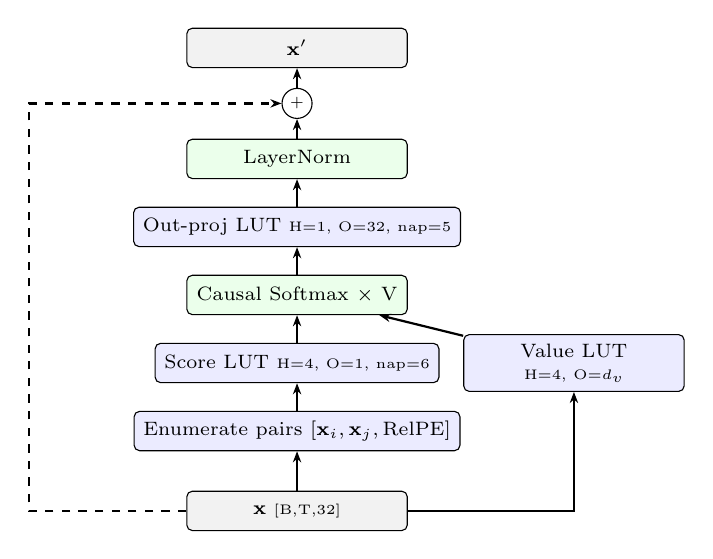
\begin{tikzpicture}[
    node distance=0.35cm,
    every node/.style={font=\scriptsize},
    block/.style={rectangle, draw, rounded corners=2pt, minimum width=2.8cm, minimum height=0.5cm, align=center, fill=#1},
    block/.default=blue!8,
    op/.style={block=green!8},
    arr/.style={-{Stealth[length=4pt]}, thick},
]
    \node[block=gray!10] (x) {$\mathbf{x}$ {\tiny[B,T,32]}};
    \node[block, above=0.5cm of x] (pairs) {Enumerate pairs $[\mathbf{x}_i, \mathbf{x}_j, \text{RelPE}]$};
    \node[block, above=of pairs] (score) {Score LUT {\tiny H=4, O=1, nap=6}};
    \node[op, above=of score] (sm) {Causal Softmax $\times$ V};
    \node[block, above=of sm] (op) {Out-proj LUT {\tiny H=1, O=32, nap=5}};
    \node[op, above=of op] (ln) {LayerNorm};
    \node[circle, draw, inner sep=1.5pt, above=0.25cm of ln] (add) {\tiny$+$};
    \node[block=gray!10, above=0.25cm of add] (out) {$\mathbf{x}'$};

    % Value branch on the right
    \node[block, right=0.3cm of score] (val) {Value LUT\\{\tiny H=4, O=$d_v$}};

    \draw[arr] (x) -- (pairs);
    \draw[arr] (pairs) -- (score);
    \draw[arr] (score) -- (sm);
    \draw[arr] (val) -- (sm);
    \draw[arr] (sm) -- (op);
    \draw[arr] (op) -- (ln);
    \draw[arr] (ln) -- (add);
    \draw[arr] (add) -- (out);
    \draw[arr] (x.east) -| (val.south);
    \draw[arr, dashed] (x.west) -- +(-2.0,0) |- (add.west);
\end{tikzpicture}
\caption{LUT Transformer V3 block. Blue: LUT modules; green: standard operations. The score LUT operates on all causal $(i,j)$ pairs.}
\label{fig:lut_v3}
\end{figure}

\subsection{Results}

\begin{table}[!t]
\caption{Simple LUT transformer results}
\label{tab:simple_lut}
\centering
\begin{tabular}{lrrr}
\toprule
Model & Params & Val loss & Steps \\
\midrule
LUT baseline (V1) & 191M & 1.463 & 100K \\
Minimalistic (nap=4) & 5.0M & 1.706 & 50K \\
V2 + self-excitement & 3.2M & 1.519 & 100K \\
\textbf{V3 softmax} & \textbf{6.5M} & \textbf{1.441} & \textbf{100K} \\
\midrule
Vanilla baseline & 4.9M & 1.356 & 100K \\
\bottomrule
\end{tabular}
\end{table}

The V3 architecture (Table~\ref{tab:simple_lut}) achieves 1.441, a gap of 0.085 to vanilla.
The key insight is separating ``what to attend to'' (LUT scores) from ``how to combine'' (standard softmax $\times$ values).
Among the LUT components, the \emph{out-projection} consistently dominates budget allocation sweeps --- it requires the most capacity.

\subsection{The Computational Challenge}

Computing attention scores with LUTs requires materialising all $O(T^2)$ pair embeddings and applying the LUT to each concatenated vector $[\mathbf{x}_i, \mathbf{x}_j, \mathrm{RelPE}]$.
On current GPUs this is computationally expensive, limiting the scale of experiments.
However, on specialised hardware with native comparator and table-read support, this pairwise operation could be strongly optimised.


% ======================================================================
\section{Ranking Attention}
\label{sec:rank_attn}

The most promising branch of our investigation replaces the LUT-based score computation with \emph{Ranking Attention}, which enables standard scaled dot-product attention on permutation features.

\subsection{From Kendall-\texorpdfstring{$\tau$}{tau} to Cosine Similarity}

Given an input $\mathbf{x} \in \mathbb{R}^d$, we define its \emph{rank signature} as the vector of $M = \binom{d}{2}$ pairwise comparisons:
\begin{equation}
    r_m(\mathbf{x}) = \mathrm{sgn}(x_{a_m} - x_{b_m}) \in \{-1, +1\}, \quad m = 1, \ldots, M
    \label{eq:rank_sig}
\end{equation}
where $(a_m, b_m)$ are fixed pairs from the upper triangle.

The Kendall-$\tau$ correlation~\eqref{eq:kendall} between two inputs is then proportional to the cosine similarity of their rank signatures:
\begin{equation}
    \tau(\mathbf{x}, \mathbf{y}) = \frac{\mathbf{r}(\mathbf{x})^\top \mathbf{r}(\mathbf{y})}{M}.
    \label{eq:tau_cosine}
\end{equation}

This means that \emph{standard scaled dot-product attention on rank features computes permutation-based similarity}.
We can use the highly optimised SDPA implementations available on modern GPUs while operating entirely on permutation features.

\subsection{Architecture}

The Ranking Attention transformer uses the following per-block structure:
\begin{enumerate}
    \item \textbf{Q, K projection:} Apply a MultiHeadLut to $(\mathbf{x} + \mathbf{p}_\mathrm{pos})$, producing queries and keys of dimension $d_{qk}$ per head.
    \item \textbf{V projection:} Apply a MultiHeadLut to $\mathbf{x}$, producing values of dimension $d_v$ per head.
    \item \textbf{Attention:} Standard causal SDPA on (Q, K, V).
    \item \textbf{Out-projection:} MultiHeadLut mapping $H \cdot d_v \to E$.
    \item \textbf{Optional FFN:} MultiHeadLut mapping $E \to E$.
    \item \textbf{Residual + LayerNorm.}
\end{enumerate}

The Q and K projections themselves are LUT-based: they map from the permutation-embedding domain (via pairwise comparisons) to a space where SDPA operates.
The attention scores are thus a function of the \emph{ordering} of input features, not their magnitudes.
The architecture is illustrated in Fig.~\ref{fig:rank_attn}.

\begin{figure}[!t]
\centering
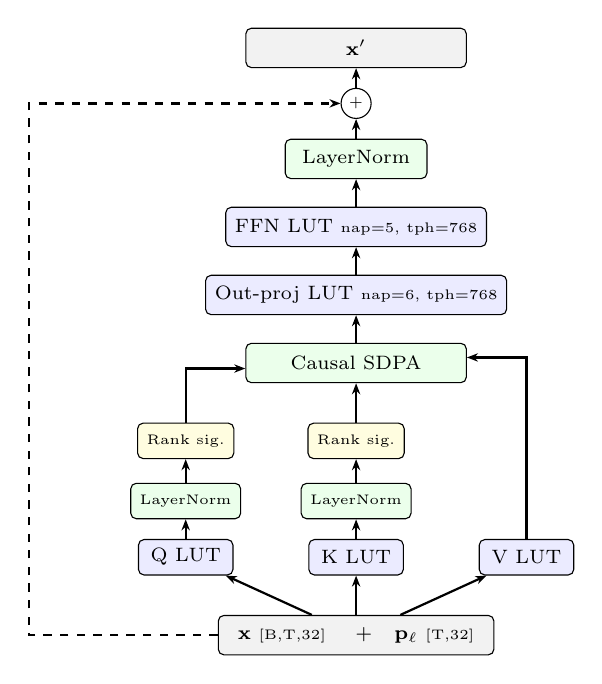
\begin{tikzpicture}[
    node distance=0.35cm,
    every node/.style={font=\scriptsize},
    block/.style={rectangle, draw, rounded corners=2pt, minimum width=2.8cm, minimum height=0.5cm, align=center, fill=#1},
    block/.default=blue!8,
    op/.style={block=green!8},
    smallblock/.style={rectangle, draw, rounded corners=2pt, minimum width=1.2cm, minimum height=0.45cm, align=center, fill=#1},
    smallblock/.default=blue!8,
    arr/.style={-{Stealth[length=4pt]}, thick},
]
    \node[block=gray!10, minimum width=3.5cm] (x) {$\mathbf{x}$ {\tiny[B,T,32]} \quad$+$\quad $\mathbf{p}_\ell$ {\tiny[T,32]}};

    % Q K V side by side
    \node[smallblock, above left=0.5cm and -0.2cm of x] (q) {Q LUT};
    \node[smallblock, above=0.5cm of x] (k) {K LUT};
    \node[smallblock, above right=0.5cm and -0.2cm of x] (v) {V LUT};

    % LN
    \node[smallblock=green!8, above=0.25cm of q, minimum width=1.0cm] (qn) {\tiny LayerNorm};
    \node[smallblock=green!8, above=0.25cm of k, minimum width=1.0cm] (kn) {\tiny LayerNorm};

    % Rank signature
    \node[smallblock=yellow!12, above=0.3cm of qn, minimum width=1.2cm] (qr) {\tiny Rank sig.};
    \node[smallblock=yellow!12, above=0.3cm of kn, minimum width=1.2cm] (kr) {\tiny Rank sig.};

    % SDPA
    \node[op, above=0.5cm of kr, minimum width=2.8cm] (sdpa) {Causal SDPA};

    \node[block, above=of sdpa] (op) {Out-proj LUT {\tiny nap=6, tph=768}};
    \node[block, above=of op] (ffn) {FFN LUT {\tiny nap=5, tph=768}};
    \node[op, above=of ffn, minimum width=1.8cm] (ln) {LayerNorm};
    \node[circle, draw, inner sep=1.5pt, above=0.25cm of ln] (add) {\tiny$+$};
    \node[block=gray!10, above=0.25cm of add] (out) {$\mathbf{x}'$};

    \draw[arr] (x) -- (q);
    \draw[arr] (x) -- (k);
    \draw[arr] (x) -- (v);
    \draw[arr] (q) -- (qn);
    \draw[arr] (k) -- (kn);
    \draw[arr] (qn) -- (qr);
    \draw[arr] (kn) -- (kr);
    \draw[arr] (qr.north) |- ([yshift=-2pt]sdpa.west);
    \draw[arr] (kr) -- (sdpa);
    \draw[arr] (v.north) |- ([yshift=2pt]sdpa.east);
    \draw[arr] (sdpa) -- (op);
    \draw[arr] (op) -- (ffn);
    \draw[arr] (ffn) -- (ln);
    \draw[arr] (ln) -- (add);
    \draw[arr] (add) -- (out);
    \draw[arr, dashed] (x.west) -- +(-2.4,0) |- (add.west);
\end{tikzpicture}
\caption{Ranking Attention block. Q and K are projected via LUTs, normalised, and mapped to rank signatures (pairwise comparisons). SDPA on rank signatures computes Kendall tau similarity.}
\label{fig:rank_attn}
\end{figure}

\subsection{Key Design Choices}

\begin{itemize}
    \item \textbf{Positional encoding:} Per-layer learned positional embeddings added to Q/K input. Summation works here because the LUT projection is itself comparison-based and tolerant of additive shifts.
    \item \textbf{Q/K budget:} Surprisingly small nap and tph suffice for Q/K (nap=3, tph=64), while out-projection and FFN need heavy capacity (nap=5--6, tph=768).
    \item \textbf{LayerNorm on Q/K:} Adding LayerNorm after Q/K projection improves stability.
    \item \textbf{GELU unembedder:} A two-layer MLP unembedder ($E \to 128 \to V$) with GELU activation outperforms a single linear layer.
\end{itemize}

\subsection{Results}

\begin{table}[!t]
\caption{Ranking Attention results}
\label{tab:rank_attn}
\centering
\begin{tabular}{llrrr}
\toprule
Exp & Description & Params & Val loss & Steps \\
\midrule
197 & RankAttn V2, clean & 6.3M & 1.505 & 50K \\
198 & + LN + heavy OP & 7.9M & 1.472 & 100K \\
207 & Optimal budget & 17.7M & 1.408 & 100K \\
208 & + pos\_dim=32 & 8.3M & 1.426 & 100K \\
225 & nap=10, tph=128 & 125.9M & \textbf{1.381} & 50K \\
\midrule
002 & Vanilla baseline & 4.9M & 1.356 & 100K \\
\bottomrule
\end{tabular}
\end{table}

The Ranking Attention architecture (Table~\ref{tab:rank_attn}) substantially outperforms simple LUT transformers.
The best result (exp225, nap=10) reaches \textbf{1.381}, within 0.025 of the vanilla baseline --- demonstrating that permutation-based representations can essentially match magnitude-based ones for this task.

However, this comes at a cost: 125.9M parameters (26$\times$ vanilla), because each table with nap=10 stores $2^{10} = 1024$ entries.
The more parameter-efficient exp208 reaches 1.426 with 8.3M parameters (1.7$\times$ vanilla), and exp207 achieves 1.408 at 17.7M (3.6$\times$ vanilla).

The remaining gap between LUT and vanilla models appears to be \emph{representational rather than optimisational}: gradient analysis shows balanced gradient-to-weight ratios across components, and attention entropy analysis reveals that LUT-based attention produces less sharp distributions than vanilla attention.


% ======================================================================
\section{HyperLUT}
\label{sec:hyperlut}

The weight overhead of standard LUT tables motivates an alternative approach.

\subsection{Motivation}

A MultiHeadLut with nap anchor pairs stores $2^{\mathrm{nap}}$ entries per table.
As nap grows to improve expressiveness, the table size grows exponentially.
This creates a tension: the best validation losses require nap=10+ (Sec.~\ref{sec:rank_attn}), but each such table carries 1024+ weight vectors.

\subsection{Architecture}

A \emph{HyperLUT} replaces the discrete table lookup with a continuous two-layer MLP operating on binary comparison features:

\begin{enumerate}
    \item \textbf{Compare:} Compute $M$ pairwise comparisons, producing binary features $c_m = \mathbf{1}[x_{a_m} > x_{b_m}] \in \{0, 1\}$.
    The forward pass uses hard (binary) comparisons; the backward pass uses a smooth surrogate (sigmoid or rational function) via the straight-through estimator (STE).
    \item \textbf{Project:} Per-head linear projection $\mathbb{R}^M \to \mathbb{R}^{h}$ (each head has its own $M$ pairs and its own weight matrix).
    \item \textbf{Activate:} ReLU (or optionally LayerNorm + ReLU).
    \item \textbf{Output:} Linear projection $\mathbb{R}^{h} \to \mathbb{R}^{n_\mathrm{out}}$.
\end{enumerate}

By design, the only information visible to a HyperLUT is the \emph{relative ordering} of input dimensions --- the binary comparison results.
Scaling all inputs by a constant changes nothing.
Yet the module uses standard matrix multiplications internally, enabling efficient GPU execution.
The HyperLUT module is illustrated in Fig.~\ref{fig:hyperlut}.

\begin{figure}[!t]
\centering
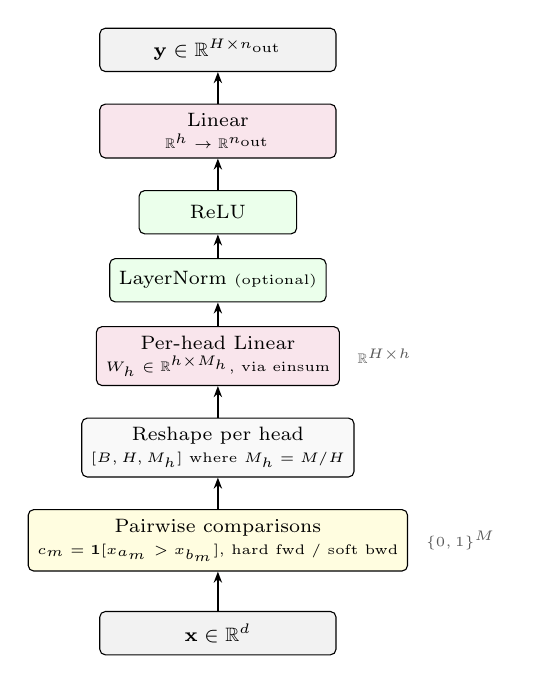
\begin{tikzpicture}[
    node distance=0.4cm,
    block/.style={rectangle, draw, rounded corners=2pt, minimum width=3.0cm, minimum height=0.55cm, font=\scriptsize, align=center, fill=#1},
    block/.default=blue!8,
    op/.style={block=green!8},
    arr/.style={-{Stealth[length=4pt]}, thick},
    lbl/.style={font=\tiny, text=gray!70!black, anchor=west},
]
    % Input
    \node[block=gray!10] (x) {$\mathbf{x} \in \mathbb{R}^d$};

    % Comparisons
    \node[block=yellow!12, above=0.5cm of x] (cmp) {Pairwise comparisons\\{\tiny $c_m = \mathbf{1}[x_{a_m} > x_{b_m}]$, hard fwd / soft bwd}};
    \node[lbl, right=0.1cm of cmp] {$\{0,1\}^{M}$};

    % Reshape
    \node[block=gray!5, above=0.4cm of cmp, minimum width=3.0cm] (reshape) {Reshape per head\\{\tiny $[B, H, M_h]$ where $M_h = M/H$}};

    % fc1 per head
    \node[block=purple!10, above=0.4cm of reshape] (fc1) {Per-head Linear\\{\tiny $W_h \in \mathbb{R}^{h \times M_h}$, via einsum}};
    \node[lbl, right=0.1cm of fc1] {$\mathbb{R}^{H \times h}$};

    % Optional LN
    \node[op, above=0.3cm of fc1, minimum width=2.0cm] (ln) {LayerNorm {\tiny(optional)}};

    % ReLU
    \node[op, above=0.3cm of ln, minimum width=2.0cm] (relu) {ReLU};

    % fc2
    \node[block=purple!10, above=0.4cm of relu] (fc2) {Linear\\{\tiny $\mathbb{R}^h \to \mathbb{R}^{n_\mathrm{out}}$}};

    % Output
    \node[block=gray!10, above=0.4cm of fc2] (out) {$\mathbf{y} \in \mathbb{R}^{H \times n_\mathrm{out}}$};

    % Arrows
    \draw[arr] (x) -- (cmp);
    \draw[arr] (cmp) -- (reshape);
    \draw[arr] (reshape) -- (fc1);
    \draw[arr] (fc1) -- (ln);
    \draw[arr] (ln) -- (relu);
    \draw[arr] (relu) -- (fc2);
    \draw[arr] (fc2) -- (out);

\end{tikzpicture}
\caption{HyperLUT module. Binary comparison features are projected per-head through a two-layer MLP. Each head has its own set of $M_h$ pairs and its own fc1 weights.}
\label{fig:hyperlut}
\end{figure}

\subsection{Preliminary Results}

\begin{table}[!t]
\caption{HyperLUT results (preliminary)}
\label{tab:hyperlut}
\centering
\begin{tabular}{llrrr}
\toprule
Exp & Description & Params & Val loss & Steps \\
\midrule
193 & HyperLUT V3 softmax & 2.3M & 1.657 & 25K \\
199 & HyperLUT + RankAttn & 4.3M & 1.513 & 100K \\
227 & HyperLUT transformer & $\sim$15M & 1.462 & 50K \\
\midrule
002 & Vanilla baseline & 4.9M & 1.356 & 100K \\
\bottomrule
\end{tabular}
\end{table}

HyperLUT results are promising but this line of investigation remains in progress (Table~\ref{tab:hyperlut}).
The best result (1.462) uses substantially fewer parameters than the best standard LUT (1.381 at 126M) while maintaining permutation semantics.

\subsection{Future Direction: HyperLUT-to-LUT Distillation}

An intriguing possibility is to \emph{train} with HyperLUTs --- exploiting fast GPU matrix multiplications and smooth gradients --- and then \emph{distil} the trained model into standard LUT tables for deployment on specialised hardware.
A HyperLUT computes a deterministic function from binary inputs to real outputs; one could in principle enumerate all $2^M$ input patterns and construct the equivalent LUT entries, or find an optimal set of smaller LUTs that approximate the HyperLUT function.
We leave this direction for future work.


% ======================================================================
\section{Discussion}
\label{sec:discussion}

\subsection{What We Have Shown}

Permutation-based transformers can approach the quality of standard magnitude-based transformers on byte-level language modelling.
The gap narrows from 0.085 (simple LUT) to 0.052 (Ranking Attention, parameter-efficient) to 0.025 (Ranking Attention, high-capacity).
The transformer structure itself --- attention, residual connections, softmax --- transfers directly; only the embedding language and projection mechanism change.

\subsection{The Weight Problem}

The central challenge is parameter efficiency.
Standard LUT tables store $2^{\mathrm{nap}} \times n_\mathrm{out}$ weights per table, and the best results require many tables with nap=10+.
Our best model (val loss 1.381) uses 26$\times$ more parameters than vanilla.
However, the \emph{inference-time bandwidth} is much lower: each table reads a single row per input, versus the dense matrix-vector products of standard transformers.

This suggests that the right metric for LUT-based models is not parameter count but \emph{bandwidth} --- the number of weight values accessed per forward pass.
On hardware with large on-chip memory and native comparator support, the LUT approach could offer significant efficiency advantages.

\subsection{Key Findings}

\begin{enumerate}
    \item \textbf{Architecture matters more than scale.} The transition from simple LUT (1.441) to Ranking Attention (1.408) was the largest improvement, not parameter scaling.
    \item \textbf{Many small tables beat few large ones} for validation loss, but large tables offer lower bandwidth.
    \item \textbf{Out-projection dominates budget.} Q/K projections can be tiny (nap=3, tph=64); the output mixing layer needs the most capacity.
    \item \textbf{Full-coverage pair sampling} consistently outperforms random sampling of anchor pairs.
    \item \textbf{Concatenated positional encoding} is essential at low embedding dimensions; additive encoding destroys ordering structure.
    \item \textbf{The gap appears representational}, not optimisational: gradient analysis shows balanced training dynamics.
\end{enumerate}


% ======================================================================
\section{Scaling to Larger Contexts}
\label{sec:scaling}

The experiments presented so far use a context length of $T = 32$ tokens, which is far shorter than production language models.
Scaling to larger contexts is the most important next step for this line of research.

We plan to evaluate the best architectures from Sections~\ref{sec:rank_attn} and~\ref{sec:hyperlut} on the nanoGPT benchmark~\cite{ref:nanogpt} with context lengths of 256--1024 tokens.
The bandwidth advantages of LUT-based models should become more pronounced at scale, as the number of table reads grows linearly with sequence length while the total table storage remains fixed.

This section will be completed in a future revision of this paper.


% ======================================================================
\section{Related Work}
\label{sec:related}

\textbf{Spiking neural networks and polychronisation.}
The theoretical foundation for this work is the Spiking Manifesto~\cite{ref:manifesto}, which builds on earlier work on polychronous groups in spiking networks~\cite{ref:polychrony}.
Our LUT formulation abstracts away the biological neuron dynamics, retaining only the essential computation: pairwise comparisons producing binary indices into weight tables.

\textbf{Locality-sensitive hashing.}
The LUT index function $H(\mathbf{x})$ partitions input space into $2^{n_c}$ buckets via hyperplane comparisons, closely related to LSH~\cite{ref:lsh}.
However, our tables are \emph{learned} end-to-end with surrogate gradients, unlike fixed hash functions.

\textbf{Multiplication-free neural networks.}
Several works have explored replacing multiplications with additions, shifts, or binary operations~\cite{ref:addernn}.
Our approach is complementary: LUT lookup is an extreme form of multiplication elimination, using only comparisons and table reads.


% ======================================================================
\section{Conclusion}
\label{sec:conclusion}

We have demonstrated that transformers can operate on permutation embeddings using lookup tables and achieve language modelling quality approaching that of standard magnitude-based transformers.
The Ranking Attention architecture, which bridges permutation-based features with efficient SDPA, reaches within 0.025 of a vanilla baseline on byte-level language modelling.

The key remaining challenge is parameter efficiency: the best LUT models require substantially more parameters than vanilla, though their inference-time bandwidth is much lower.
HyperLUT offers a promising path toward bridging this gap by combining permutation semantics with GPU-friendly matrix multiplications.

More broadly, this work shows that the \emph{relative ordering} of embedding dimensions carries rich representational capacity --- enough to support competitive sequence modelling.
This opens pathways toward specialised hardware that replaces multiply-accumulate units with comparators and table reads, potentially offering substantial energy and latency improvements.


% ======================================================================
\section*{Acknowledgment}

The authors thank Mikhail Burtsev for valuable discussions and feedback.


% ======================================================================
\begin{thebibliography}{99}

\bibitem{ref:manifesto}
E.~Izhikevich, ``Spiking Manifesto,'' arXiv:2512.11843, Dec.~2025.

\bibitem{ref:vaswani}
A.~Vaswani, N.~Shazeer, N.~Parmar, J.~Uszkoreit, L.~Jones, A.~N.~Gomez, \L.~Kaiser, and I.~Polosukhin,
``Attention is all you need,'' in \emph{Proc.\ NeurIPS}, 2017.

\bibitem{ref:fineweb}
G.~Penedo, H.~Malartic, D.~Hesslow, R.~Cojocaru, A.~Cappelli, H.~Alobeidli, B.~Pannier, E.~Almazrouei, and J.~Launay,
``The FineWeb Datasets: Decanting the Web for the Finest Text Data at Scale,'' arXiv:2406.17557, 2024.

\bibitem{ref:adam}
D.~P.~Kingma and J.~Ba, ``Adam: A method for stochastic optimization,'' in \emph{Proc.\ ICLR}, 2015.

\bibitem{ref:polychrony}
E.~M.~Izhikevich, ``Polychronization: Computation with spikes,'' \emph{Neural Computation}, vol.~18, no.~2, pp.~245--282, 2006.

\bibitem{ref:lsh}
A.~Andoni and P.~Indyk, ``Near-optimal hashing algorithms for approximate near neighbor in high dimensions,'' in \emph{Proc.\ FOCS}, 2006.

\bibitem{ref:addernn}
H.~Chen, Y.~Wang, C.~Xu, B.~Shi, C.~Xu, Q.~Tian, and C.~Xu,
``AdderNet: Do we really need multiplications in deep learning?,'' in \emph{Proc.\ CVPR}, 2020.

\bibitem{ref:nanogpt}
A.~Karpathy, ``nanoGPT,'' \url{https://github.com/karpathy/nanoGPT}, 2023.

\end{thebibliography}

\end{document}
